\section{Technology and infrastructure (as-is)}
\label{sec:as-is}

LowTech GmbH as-is infrastructure:
\begin{figure}[H]
\centering
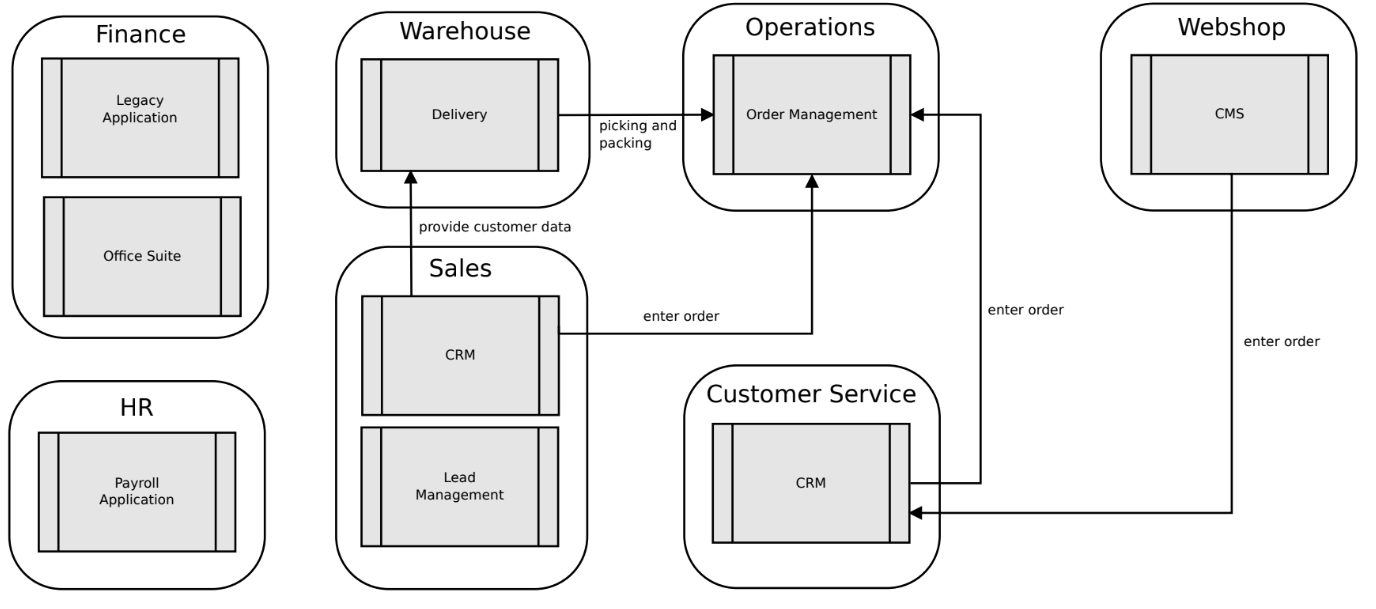
\includegraphics[width=1\textwidth]{Images/LowTech} 
\caption{Application landscape of Low Tech GmbH, showing key systems and their integrations.}
\label{fig:vite}
\end{figure}

\subsection{Server Resources}
\label{sec:server_res}

Table~\ref{tab:resources} shows the total server resources allocated across different departments.

\begin{table}[h!]
\centering
\begin{tabular}{llccc}
\toprule
\textbf{Department} & \textbf{RAM} & \textbf{Storage (HDD)} & \textbf{Storage (SSD)} & \textbf{Storage (Tape Drive)} \\
\midrule
Finance   & 8GB   & 500GB  & -    & -      \\
HR        & 8GB   & 2000GB & -    & -      \\
Warehouse & 8GB   & 1000GB & -    & -      \\
Sales     & 16GB  & 2000GB & -    & -      \\
Sales     & 32GB  & -      & -    & 10000GB \\
Operations & 32GB & 3000GB & -    & -      \\
Webshop   & 128GB & -      & 500GB & -      \\
\midrule
\textbf{Total}       & \textbf{232GB} & \textbf{8500GB} & \textbf{500GB} & \textbf{10000GB} \\
\bottomrule
\end{tabular}
\caption{Server resources allocated by department (summed up).}
\label{tab:resources}
\end{table}

\newpage
\subsection{Traffic and usage (last month)}
\label{sec:traffic}

\begin{table}[h!]
\centering
\begin{tabular}{llccc}
\toprule
\textbf{System/Service} & \textbf{Storage Used} \\
\midrule
Legacy Accounting Software & 350GB \\  
Payroll                   & 1000GB \\  
Delivery                  & 250GB \\  
CRM                       & 980GB \\  
CRM Storage               & 5500GB \\  
Order Management          & 100GB \\  
CMS                       & 10GB \\  
\midrule
\textbf{Total}            & \textbf{8190GB} \\  
\bottomrule
\end{tabular}
\caption{Server resources allocated by department (summed up).}
\label{tab:resources}
\end{table}

The infrastructure of Low Tech GmbH consists of various systems and departmental allocations, with a total of 232 GB RAM, 8500 GB HDD, 500 GB SSD, and 10,000 GB of tape drive storage. Storage utilization over the past month amounted to 8190 GB, with CRM and payroll systems being the primary consumers.

\newpage
\subsection{Power consumption)}
\label{sec:power}

\textbf{Servers:}
\begin{table}[h!]
\centering
\begin{tabular}{llccc}
\toprule
\textbf{Type} & \textbf{Amount} & \textbf{Electricity Consumption (Per Server)} & \textbf{Total Consumption} \\
\midrule
Application Server & 4 & 1000W & 4000W \\
Application Server & 1 & 1200W & 1200W \\
Storage Server     & 1 & 1200W & 1200W \\
Web Server         & 1 & 1200W & 1200W \\
\midrule
\textbf{Total}     & 7 &        & \textbf{7600W} \\
\bottomrule
\end{tabular}
\caption{Power consumption by server type (summed up).}
\label{tab:Power_server}
\end{table}


The calculation of the monthly energy consumption is as follows:

\begin{equation}
\frac{7600 \, \text{W}}{1000} = 7.6 \, \text{kW}
\end{equation}

The monthly energy consumption is calculated by:

\begin{equation}
7.6 \, \text{kW} \times 24 \, \text{h} \times 30 \, \text{days} = 5472 \, \text{kWh} \, \text{per month}
\end{equation}


\textbf{Clients:}
\begin{table}[h!]
\centering
\begin{tabular}{llccc}
\toprule
\textbf{Type} & \textbf{Amount} & \textbf{Electricity Consumption (Per Unit)} & \textbf{Total Consumption} \\
\midrule
Clients & 17 & 500W & 8500W \\
Laptops & 14 & 50W & 700W \\
Laptops & 5 & 1 & 100W & 500W \\
\midrule
\textbf{Total}     & 7 &        & \textbf{9700W} \\
\bottomrule
\end{tabular}
\caption{Power consumption by server type (summed up).}
\label{tab:Power_client}
\end{table}

\begin{equation}
\frac{9700 \, \text{W}}{1000} = 9.7 \, \text{kW}
\end{equation}

For the client energy consumption:

\begin{equation}
9.7 \, \text{kW} \times 8 \, \text{hours} \times 21 \, \text{days} = 1629.6 \, \text{kWh} \, \text{per month}
\end{equation}

The total energy consumption per month is:

\begin{equation}
5472 \, \text{kWh} \, (\text{Servers}) + 1629.6 \, \text{kWh} \, (\text{Clients}) = 7101.6 \, \text{kWh} \, \text{per month}
\end{equation}

The energy demand is significant, with server usage accounting for 5472 kWh per month across seven servers, predominantly driven by application and web servers. Client devices, including 17 desktop clients and 19 laptops, contribute an additional 1629.6 kWh per month. Overall, the monthly energy consumption totals 7101.6 kWh.

\subsection{Critical assessment)}
\label{sec:critical_assessment}

\begin{itemize}
    \item \textbf{Scalability}
    \begin{itemize}
        \item Old Hardware
        \item No space for more Hardware
    \end{itemize}
    
    \item \textbf{Availability}
    \begin{itemize}
        \item No redundancy
        \item No UPS (Uninterruptible Power Supply)
    \end{itemize}
    
    \item \textbf{Security}
    \begin{itemize}
        \item Only Windows Defender and pfSense
        \item No Role-based Access Controls
        \item Maybe lack in encryption
        \item Outdated platforms and software
    \end{itemize}
\end{itemize}

The current infrastructure lacks scalability, security, and high availability, falling short of modern standards. Immediate upgrades are essential to ensure system resilience, enhanced security, and capacity for future growth.





